\documentclass[border=3pt,tikz]{standalone}
\usepackage{amsmath,amssymb}
\usepackage{siunitx}
\usepackage{tikz}
\usepackage[outline]{contour} % glow around text
\tikzset{>=latex}
\contourlength{1.1pt}

\colorlet{mycyan}{blue!20!cyan!40!black}
\colorlet{myred}{red!40!black}
\colorlet{mydarkblue}{blue!40!black}
\colorlet{myblue}{blue!65!black}
\colorlet{mygreen}{green!60!black}

\begin{document}


% TEMPERATURE SCALE
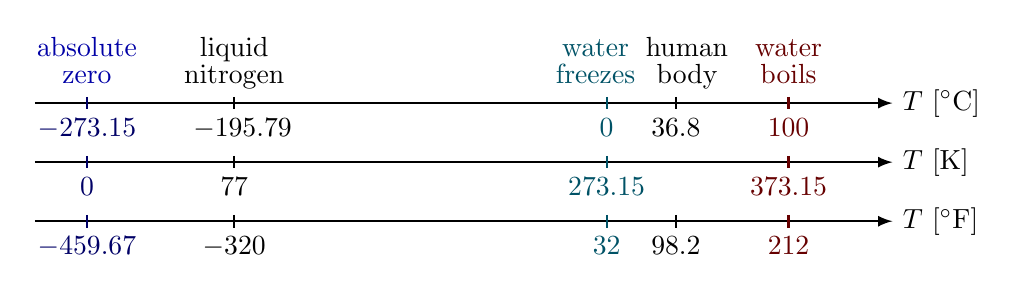
\begin{tikzpicture}[xscale=1.1]
  \def\Tzero{-6.0}  % absolute zero
  \def\Tnitro{-4.3} % liquid nitrogen
  \def\Tbody{0.8}   % body temperature
  \def\Tboil{2.1}   % boiling temperature
  \def\Tmax{3.0}    % maximum temperature on the scale
  \def\h{0.75}      % axis off sets
  \def\tick#1#2#3{\draw[thick,#3] (#1+.08) --++ (0,-.16) node[below=-.5pt,scale=1] {#2};}
  
  % AXIS
  \draw[->,thick] % degrees Celsius
    (1.1*\Tzero,0) -- (1.1*\Tmax,0) node[right] {$T$ [$^\circ$C]};
  \draw[->,thick] % Kelvin
    (1.1*\Tzero,-\h) -- (1.1*\Tmax,-\h) node[right] {$T$ [K]};
  \draw[->,thick] % Fahrenheit
    (1.1*\Tzero,-2*\h) -- (1.1*\Tmax,-2*\h) node[right] {$T$ [$^\circ$F]};
  
  % LABEL
  \node[above=-3,align=center,myblue] at (\Tzero,0.1) {absolute\\[-2]\strut zero};
  \node[above=-3,align=center] at (\Tnitro,0.1) {liquid\\[-2]\strut nitrogen};
  \node[left=4,above=-3,align=center,mycyan] at (0,0.1) {water\\[-2]\strut freezes};
  \node[right=4,above=-3,align=center] at (\Tbody,0.1) {human\\[-2]\strut body};
  \node[above=-3,align=center,myred] at (\Tboil,0.1) {water\\[-2]\strut boils};
  
  % CELSIUS
  \tick{\Tzero,0}{$-273.15$}{mydarkblue} % absolute zero
  \tick{\Tnitro,0}{\hspace{6pt}$-195.79$}{} % liquid nitrogen
  \tick{0,0}{0}{mycyan}              % freezing temperature
  \tick{\Tbody,0}{36.8}{}            % body temperature
  \tick{\Tboil,0}{100}{myred}        % boiling temperature
  
  % KELVIN
  \tick{\Tzero,-\h}{0}{mydarkblue}   % absolute zero
  \tick{\Tnitro,-\h}{77}{}           % liquid nitrogen
  \tick{0,-\h}{273.15}{mycyan}       % freezing temperature
  %\tick{\Tbody,-\h}{310.0}{}        % body temperature
  \tick{\Tboil,-\h}{373.15}{myred}   % boiling temperature
  
  % FAHRENHEIT
  \tick{\Tzero,-2*\h}{$-459.67$}{mydarkblue} % absolute zero
  \tick{\Tnitro,-2*\h}{$-320$}{}      % liquid nitrogen
  \tick{0,-2*\h}{32}{mycyan}          % freezing temperature
  \tick{\Tbody,-2*\h}{98.2}{}         % body temperature
  \tick{\Tboil,-2*\h}{212}{myred}     % boiling temperature
  
\end{tikzpicture}


% TEMPERATURE SCALE
%   K = C + 273.15
%   F = 1.8*C - 32
%   T_intersection = (32-273.15)/(1-1.8) = 301.44
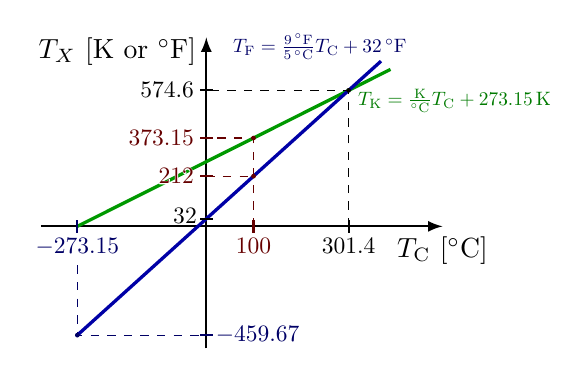
\begin{tikzpicture}
  \def\xmin{-2.1}
  \def\xmax{3.0}
  \def\ymin{-1.55}
  \def\ymax{2.4}
  \def\xs{0.006}  % x scale
  \def\ys{0.003} % y scale
  \def\Tmin{-273.15}
  \def\Tmax{390}
  \def\TF#1{(1.8*(#1)+32)}
  \def\xtick#1#2{\draw[thick,#2] (\xs*#1,.08) --++ (0,-.16) node[below=-1,scale=0.85] {$#1$};}
  \def\ytick#1#2{\draw[thick,#2] (.08,\ys*#1) --++ (-.16,0) node[left=-1,scale=0.85] {\contour{white}{$#1$}};}
  
  % AXIS
  \draw[->,thick] (\xmin,0) -- (\xmax,0) node[below] {$T_\text{C}$ [$^\circ$C]};
  \draw[->,thick] (0,\ymin) -- (0,\ymax) node[below=5,left=0] {$T_X$ [K or $^\circ$F]};
  
  % CURVES
  \draw[very thick,mygreen]
    (\xs*\Tmin,0) -- (\xs*\Tmax,{\ys*(\Tmax+273.15)})
    node[pos=0.89,below right=-2,scale=0.7,mygreen!80!black]
      {$T_\text{K} = \frac{\si{K}}{\si{\degree C}} T_\text{C}+\SI{273.15}{K}$};
  \draw[very thick,myblue] % Fahrenheit
    (\xs*\Tmin,{\ys*\TF{\Tmin}}) -- ({\xs*(\Tmax-20)},{\ys*\TF{\Tmax-20}})
    node[right=10,above left=-2,scale=0.7,mydarkblue]
      {$T_\text{F} = \frac{\SI{9}{\degree F}}{\SI{5}{\degree C}} T_\text{C}+\SI{32}{\degree F}$};
  
  % DASHED LINES
  \draw[dashed,mydarkblue]
    (\xs*\Tmin,0.32*\ymin) -- (\xs*\Tmin,{\ys*\TF{\Tmin}}) --++ (-\xs*\Tmin,0);
  \draw[dashed,myred]
    (0,\ys*212) --++ (\xs*100,0)
    (\xs*100,0) |- (0,\ys*373.15);
  \draw[dashed,black] (\xs*301.4,0) |- (0,\ys*574.6);
  \fill[myred]
    (\xs*100,\ys*212) circle(0.03)
    (\xs*100,\ys*373.15) circle(0.03);
  \fill[black,mydarkblue] (\xs*\Tmin,{\ys*\TF{\Tmin}}) circle(0.03);
  \fill[black] (\xs*301.4,\ys*574.6) circle(0.03);
  
  % TICKS
  \xtick{-273.15}{mydarkblue}
  \xtick{301.4}{black}
  \xtick{100}{myred}
  \draw[thick] (0.08,\ys*32) --++ (-0.16,0) % freezing in Fahrenheit
    node[above=1,left=-2,scale=0.85] {$32$};
  %\ytick{32}{black}     % freezing in Fahrenheit
  \ytick{212}{myred}    % water boiling in Fahrenheit
  \ytick{373.15}{myred} % water boiling in Kelvin
  \ytick{574.6}{black}
  %\ytick{-459.7}{mydarkblue}
  \draw[thick,mydarkblue] (-0.08,{\ys*\TF{\Tmin}}) --++ (0.16,0)
    node[right=-2,scale=0.85] {$-459.67$};
  
\end{tikzpicture}


\end{document}
